\subsection{The link-analysis algorithm}\label{sec:background:theory:linkanalysis}

\Warning[TODO]{ Detailed introduction/description! }

The \textit{link-analysis} algorithm, as presented by \cite{huang2004link} and further discussed in \cite{huang2007comparison}.  See the articles for more information and in-depth examples. What follows is a condensed description of how the algorithm works.

The algorithm is an adaptation of HITS \cite{kleinberg1999authoritative} which is a web page ranking algorithm to the recommendation domain. The original algorithm distinguish between \textit{Authoritative} pages which definitely contain high-quality information and \textit{Hub} pages which are comprehensive lists of links to authoritative pages. \citep{huang2007comparison}

Adaptation to the recommendation domain is achieved by introducing the \textit{product representativeness} score $\PR$ and the \textit{consumer representativeness} score $\CR$.

The \textit{product representativeness} score $\PR(i, u)$ can be seen as a measure of the item $i$'s level of interest with respect to user $u$, or in other words $i$'s authority of $u$'s interests in $i$.

The \textit{consumer representativeness} score $\CR(u, \hat{u})$ measures how well $u$ as a hub for $\hat{u}$ associates with items of interests to $\hat{u}$.

If $h_{u, i}$ is the user-item interaction history as defined by \ref{eq:hist} and $A$ is the interaction matrix then a recursive definition of the authority and hub scores can be defined as

\begin{equation}
    \PR = A' * \CR
\end{equation}

\begin{equation}
    \CR = B * \PR + \CR_0
\end{equation}

Where $B = (b_{u, i})$ is a matrix such that:

\begin{equation}
    b_{u, i} = \frac{ h_{u, i} }{ \left(\sum_{i} h_{u, i}\right)^\gamma }
\end{equation}

Meaning $B$ normalizes the representativeness score a costumer receives from linked items by dividing it with the total number of items the customer is linked to.  $\gamma$ controls the extent to which a consumer is penalized for making many purchases.

$\CR_0$ is defined as

\begin{equation}
    \CR_{i, j}^0 = \begin{cases}
        \eta \quad \text{if } \; i = j \\
        0    \quad \text{otherwise}
    \end{cases}
\end{equation}

in other words $\CR_0 = \eta * I_M$ where $I_M$ is an $M x M$ identity matrix and $M$ is the number of users.  It is included to maintain the high representativeness score for the target users themselves. This also necessitates a normalization step to keep the values on a consistent level.

In summary the \textit{link-analysis} algorithm follow these steps:

\begin{enumerate}
    \item Construct the interaction matrix $A$ and the associating matrix $B$.

    \item Set $\CR_0 = \eta * I_M$.
    \item At each iteration $t = 1, \ldots, t_{max}$ perform:

        \begin{enumerate}
            \item $\PR_t = A' * \CR_{t- 1}$
            \item $\CR_t = B * \PR_t$
            \item Normalize $\CR_t$ so each column adds up to 1
            \item $\CR_t = \CR_t + \CR_0$
        \end{enumerate}

        Repeat until convergence.

    \item Predicted user-item interaction is given by $P = \PR'$.

\end{enumerate}

There are two parameters to the algorithm: $\gamma$ and $\eta$.


\subsubsection{Runtime exmple}

This is a runtime example for \textit{link-analysis} using a simple interaction matrix \eqref{eq:exA}, corresponding to the interaction graph \figureref{fig:ex_graph}.

\begin{equation}\label{eq:exA}
  A = \kbordermatrix{
    &    i_1 & i_2 & i_3 & i_4 \\
    u_1 & 0   & 1   & 0   & 1  \\
    u_2 & 0   & 1   & 1   & 1  \\
    u_3 & 1   & 0   & 1   & 0
  }
\end{equation}

\begin{figure}[h!]
    \centering
    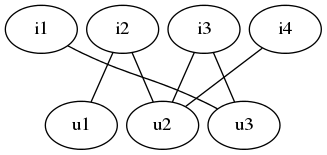
\includegraphics[width=0.3\linewidth]{fig/example_run/item_user_graph.png}
    \caption{A graph representing interactions between each user and item.}
    \label{fig:ex_graph}
\end{figure}

The following example uses $\gamma = 0.9$ and $\eta = 1$.


\[
  B = \kbordermatrix{
    &    i_1 & i_2 & i_3 & i_4 \\
    u_1 & 0         & 0.5359    & 0         & 0.5359  \\
    u_2 & 0         & 0.3720    & 0.3720    & 0.3720  \\
    u_3 & 0.5359    & 0         & 0.5359    & 0
  },
\;
  \CR_0 = \kbordermatrix{
    &    u_1 & u_2 & u_3 \\
    u_1 & 1   & 0  & 0  \\
    u_2 & 0   & 1  & 0  \\
    u_3 & 0   & 0  & 1
  }
\]

During the iterations the rows of $\PR$ will be representing each item and each column will be representing each user, this is the reverse of the interaction matrix $A$. The example therefore presents the transpose of $\PR$, $\PR'$.

\[
    \PR'_1 = \begin{pmatrix}
        0 & 1 & 0 & 1 \\
        0 & 1 & 1 & 1 \\
        1 & 0 & 1 & 0
    \end{pmatrix},
\;
    \CR_1 = \begin{pmatrix}
        1.5902 & 0.4098 & 0 \\
        0.3935 & 1.4098 & 0.1967 \\
        0      & 0.2577 & 1.7423
    \end{pmatrix}
\]

\[
    \PR'_2 = \begin{pmatrix}
             0 &  2.0000 &  0.4098 &  2.0000 \\
        0.1967 &  1.8033 &  1.6065 &  1.8033 \\
        1.7423 &  0.2577 &  2.0000 &  0.2577
    \end{pmatrix},
\;
    \CR_2 = \begin{pmatrix}
        1.5354 &  0.4098 &  0.0548 \\
        0.3994 &  1.4008 &  0.1997 \\
        0.0858 &  0.2909 &  1.6233
    \end{pmatrix}
\]

\[
    \PR'_3 = \begin{pmatrix}
        0.0548 &  1.9452 &  0.4646 &  1.9452 \\
        0.1997 &  1.8003 &  1.6006 &  1.8003 \\
        1.6233 &  0.3767 &  1.9142 &  0.3767
    \end{pmatrix},
\;
    \CR_3 = \begin{pmatrix}
        1.5234 &  0.4067 &  0.0699 \\
        0.3995 &  1.4007 &  0.1998 \\
        0.1226 &  0.3015 &  1.5759
    \end{pmatrix}
\]

After transposing $\PR$ and removing the items users already have interacted with in $A$, the prediction matrix $P$ becomes

\[
  P = \kbordermatrix{
    &    i_1 & i_2 & i_3 & i_4 \\
    u_1 &     0.0548 &  0 &  \mathbf{0.4646} &  0 \\
    u_2 &     \mathbf{0.1997} &  0 &  0 &  0 \\
    u_3 &     0 &  \mathbf{0.3767} &  0 &  \mathbf{0.3767}
  }
\]

\Figureref{fig:ex_graph_link_rec} is a visualization of the most recommended items.

\begin{figure}[h!]
    \centering
    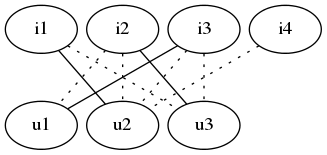
\includegraphics[width=0.3\linewidth]{fig/example_run/item_user_graph_link_rec.png}
    \caption{A graph representing the most recommended item for each user. The dotted lines represent previous interactions.}
    \label{fig:ex_graph_link_rec}
\end{figure}

\FloatBarrier

